\documentclass[11pt,a4paper]{article}
\usepackage[utf8]{inputenc}
\usepackage[T1]{fontenc}
\usepackage[spanish]{babel}
\usepackage[margin=2.5cm]{geometry}
\usepackage{graphicx}
\setlength{\parindent}{0pt}
\setlength{\parskip}{0.6em}

\begin{document}

\textbf{Declaración:} Esta es la transcripción fiel de la prueba escrita a mano el 18/11/2026; las fotografías de las hojas están en el anexo.

\bigskip
\hrule
\bigskip

Caso de estudio: Sistema de Monitoreo de la cadena de frio <<Frio Vac>>

Nombres: Cristopher Lavayen \hfill Fecha: 18/11/2026

T1. Conceptos aplicados al caso

(a) Explique con sus palabras que es un requisito según iso/iEC/IEEE 29148 y con esa explicación, decida si E7 y E12 son requisitos de producto de FRIOVAC. Justifique cada decisión en una o dos lineas

Un requisito es una necesidad la cual puede contender ciertas, restricciones. y esta puede ser documentada para posteriormente ser solucionada por un equipo de desarrollo.

E7 y E12 no son requisitos del producto ya que no resaltan ninguna necesidad para ser resuelta o documentada.

(b) Expliqué qué describe la especificación de los interesados(SIRS) la especificación de requisitos del sistema (SyRS) y la especificación de requisitos del software (SRS) en este proyecto. Para cada una dé un enunciado del insumo A que iría en ella y diga por que.

E1: Esta describe una especificación de requisito a los interesados ya que especifica una necesidad hacia los stekholder.

E2: Este describe una especificación (SyRs) habla de un componente del sistema que iva integrado.

E3: Este describe una especificación de requisitos (SyRs) habla de componentes que el sistema integrara.

E4: Este describe uno. (StRs) especifica el tiempo en que los stekholder deben desarrolar el sistema.

\clearpage

E5: Describe una especificación (SRS) ya que el sistema debe genera un PDF la cual con lleva a una funcionalidad que contiene este

E6: Describe una especificación (SRS) ya que le consta al sistema funcionar si o si dentro de ese lapso de tiempo sin luz

E7: Describe una especificación (STRS) ya que menciona el tipo de registro que lleva.

E8: El enunciado mismo lo describe que es un (SyRS) ya que menciona una funcionalidad que debe llevar el sistema.

E9: Este describe una especificacion de tipo (SRS) ya que menciona otros componentes que el sistema integrara en su entorno.

E10: Este describe una especificacion de tipo (SyRS) ya que menciona una auditoría la cual puede hacer un rol especifico

E11: Este describe una especificación de tipo (SYRS) ya que habla acerca del manejo del sistema y su interaccion y debidos proceso.

E12: Describe una especificación del tipo (STRS) ya que menciona el proceso de entrevista con un numero de interesados.

\clearpage

\appendix
\section*{Anexo: fotografías de las hojas}
\begin{center}
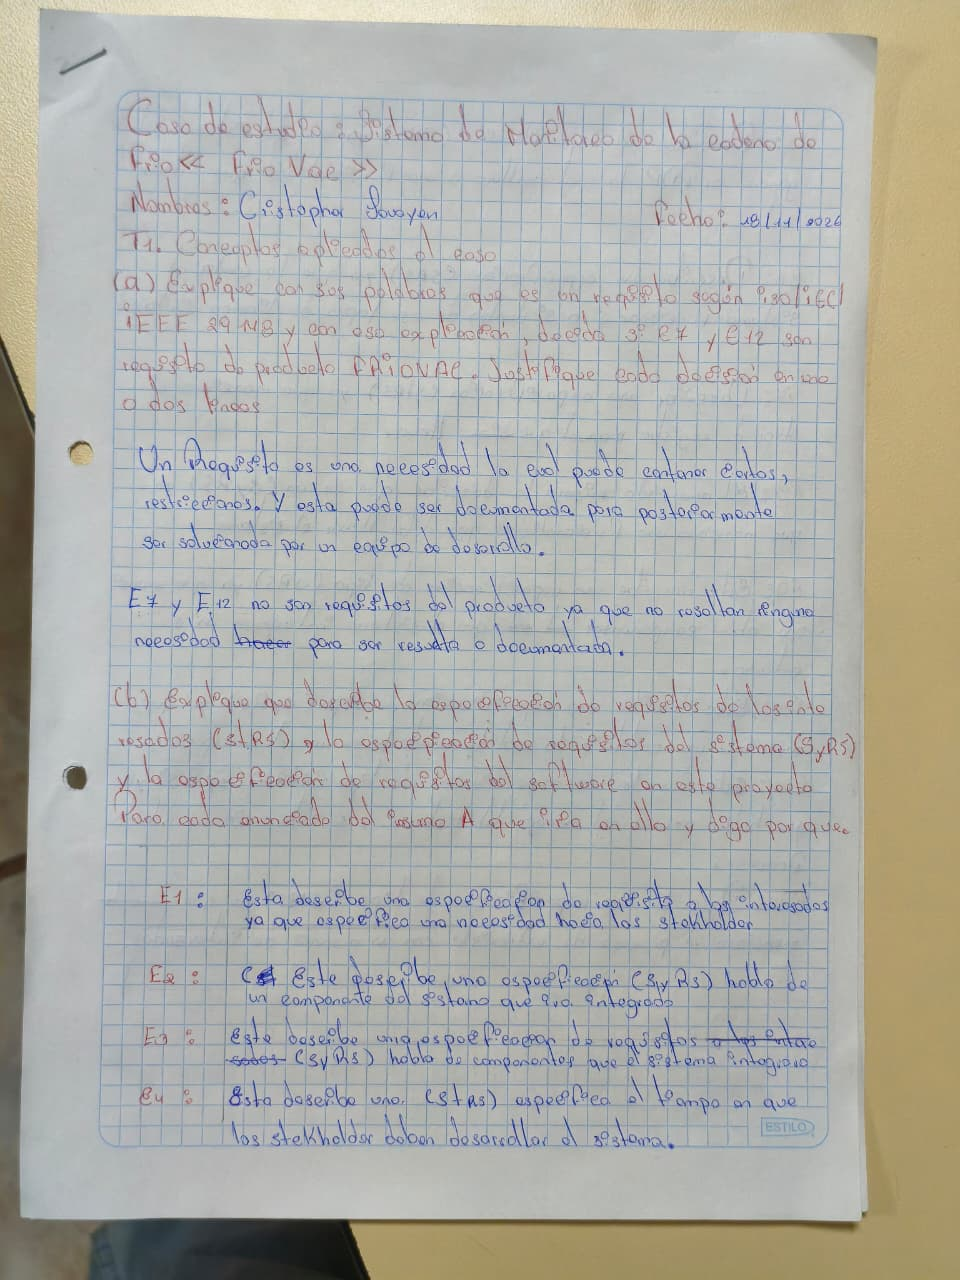
\includegraphics[width=\textwidth,height=0.8\textheight,keepaspectratio]{evidencias/hoja-01.jpeg}
\end{center}
\clearpage
\begin{center}
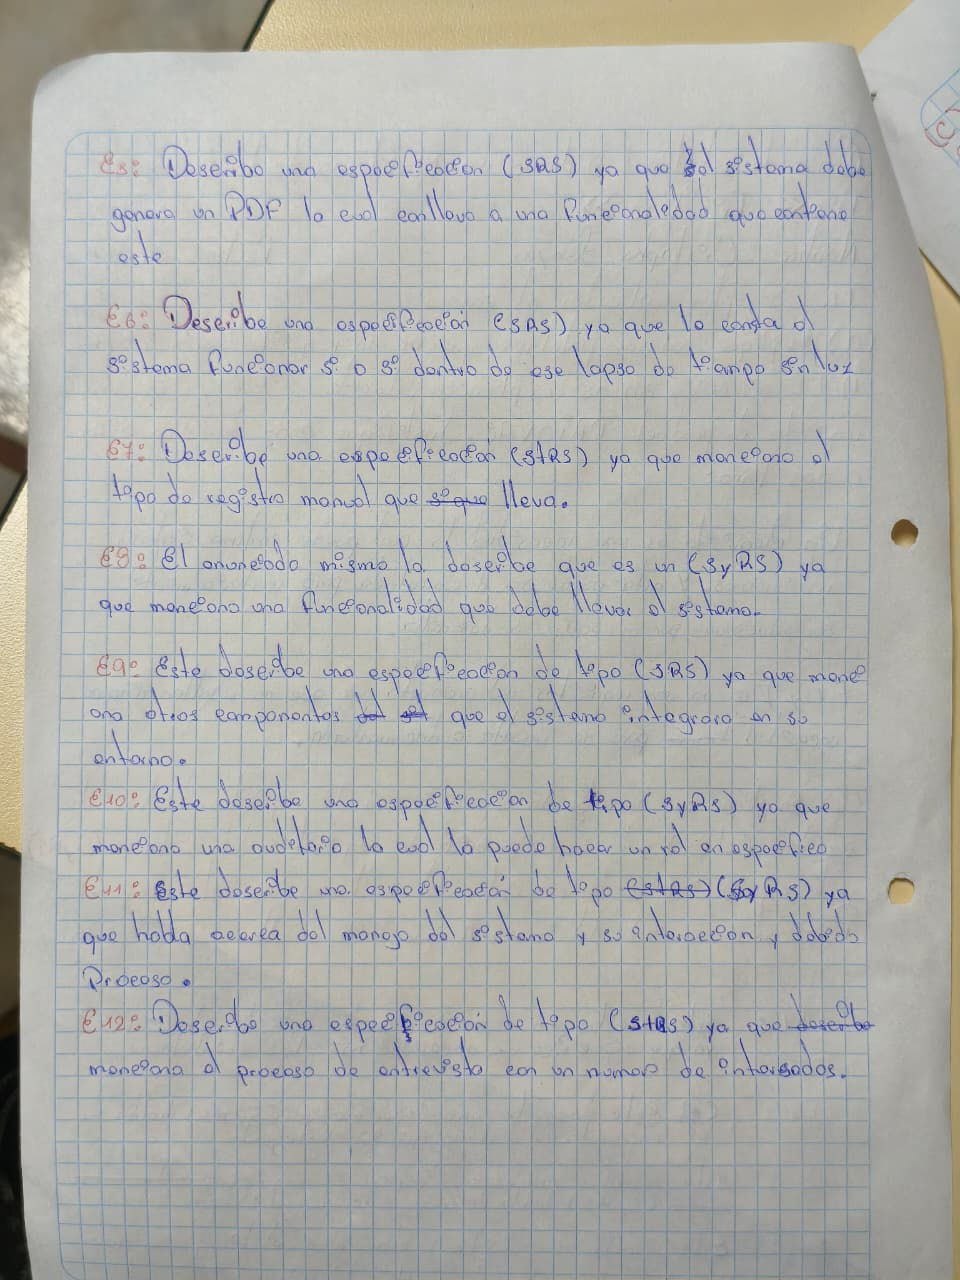
\includegraphics[width=\textwidth,height=0.85\textheight,keepaspectratio]{evidencias/hoja-02.jpeg}
\end{center}

\end{document}
